\chapter{Normalización de Flujos y Preservación de Color} \label{Metodologia:NormalizacionFlujos}

Las curvas de luz obtenidas de los catálogos Gaia y ZTF al igual que las
observaciones realizadas en el OAU permiten el estudio de \atoObjId ajustando un
modelo de un sistema binario eclipsante utilizando PHOEBE. Sin embargo, PHOEBE
trabaja directamente con flujos; al calcular el modelo hacia adelante PHOEBE
integra las intensidades calculadas para cada elemento superficial de ambas
estrellas e integra la radiación emergente en la dirección del observador para
obtener una medición del flujo en unidades de $\mathrm{W} \mathrm{m}^{-2}$. Los
datos obtenidos del catálogo de Gaia vienen con el flujo registrado por el
satélite de cada tránsito del objeto por su campo de visión\textemdash este
viene reportado en unidades de $\mathrm{e}^{-} \mathrm{s}^{-1}$, el cual se
puede utilizar directamente en PHOEBE en el caso de no necesitar conocer la
luminosidad absoluta de las componentes estelares. 

Los datos recabados del catálogo de ZTF no reportan alguna medición directa del
flujo recibido\textemdash estos solo reportan las magnitudes y sus errores
obtenidas de su procesamiento fotométrico. El procesamiento de las imágenes en
cada filtro descrito por
\citeyearparen{masci_ztf_data_processing_products_archive_2018} da como
resultado curvas de luz calibradas con estrellas de calibración del catálogo
Pan-STARRS1. Aunque no es posible obtener una medición del flujo recibido sin
conocer el flujo $f_0$ que corresponde a una magnitud $m_0$, es posible obtener
curvas de flujos normalizados que preservan la información del color del sistema
ofrecido por la fotometría multibanda. Para cada punto de magnitud $m_p$ para la
pasabanda $p$ se aplica la siguiente transformación para obtener el flujo
normalizado:

\begin{eqfloat}[!ht]
	\centering
	\begin{equation}
		f_p = 10^{-\frac{2}{5} (m_p - m_0)}
	\end{equation}
	\blankcaption
	\label{ecuacionNormalizarFlujos}
\end{eqfloat}

Donde $m_0$ es la magnitud de referencia. En vez de escoger una magnitud $m_0$
para cada pasabanda se elige solo un valor de $m_0$ el cual se aplica a ambas
curvas de ZTF, dando como resultado el flujo relativo obtenido del sistema en
base a su distribución de energía espectral (SED). Este dato permite el ajuste
de la temperatura efectiva del sistema sin necesidad de acudir a una estimación
a priori basado en relaciones analíticas o estadísticas con respecto a otros
parámetros del modelo
[\citetbooksection{kallrath_eclipsing_binary_modelling_2009}{5.1.2.2}]. A la
vez, al tener una manera concreta de evaluar de manera directa la temperatura
efectiva del sistema es posible conocer la incertidumbre utilizando solo datos
fotométricos. Para obtener el flujo normalizado de las curvas de ZTF se utilizó
la magnitud del sistema en la fase 0.25 en la pasabanda ZTF:g. El resultado se
puede ver en la \reffigure{figuraNormFlujosCurvas}. El código donde se realizó
este procedimiento se encuentra en el Notebook
\href{https://github.com/KnightIV/UANL_MAPTA_Observaciones/blob/main/analisis/ztf/light-curve-processing.ipynb}{\code{light-curve-processing.ipynb}}.

Debido a que la curva de luz de las observaciones hechas en el OAU en Iturbide,
N.L. son magnitudes diferenciales, no es posible determinar el flujo real
incidente a la CCD. Por lo tanto se adopta el mismo procedimiento hecho para las
curvas de luz de ZTF. Utilizando la \refequation{ecuacionNormalizarFlujos} los
flujos normalizados se obtuvieron usando la magnitud en fase 0.25 como el valor
de $m_0$, el código presente en el Notebook
\href{https://github.com/KnightIV/UANL_MAPTA_Observaciones/blob/main/analisis/period-analysis/periodogram.ipynb}{\code{periodogram.ipynb}}.
La curva de luz resultante se puede ver en la
\reffigure{figuraNormFlujosCurvas}. Como se mencionó al principio del capítulo,
no fue necesario tratar las curvas obtenidas de Gaia DR3 de esta manera, debido
a que los datos obtenidos de la fotometría de
época\footnote{\url{https://gea.esac.esa.int/archive/documentation/GDR3/Gaia_archive/chap_datamodel/sec_dm_photometry/ssec_dm_epoch_photometry.html}}
ya reporta el flujo medido por Gaia. 

\begin{figure}[!ht]
	\centering
	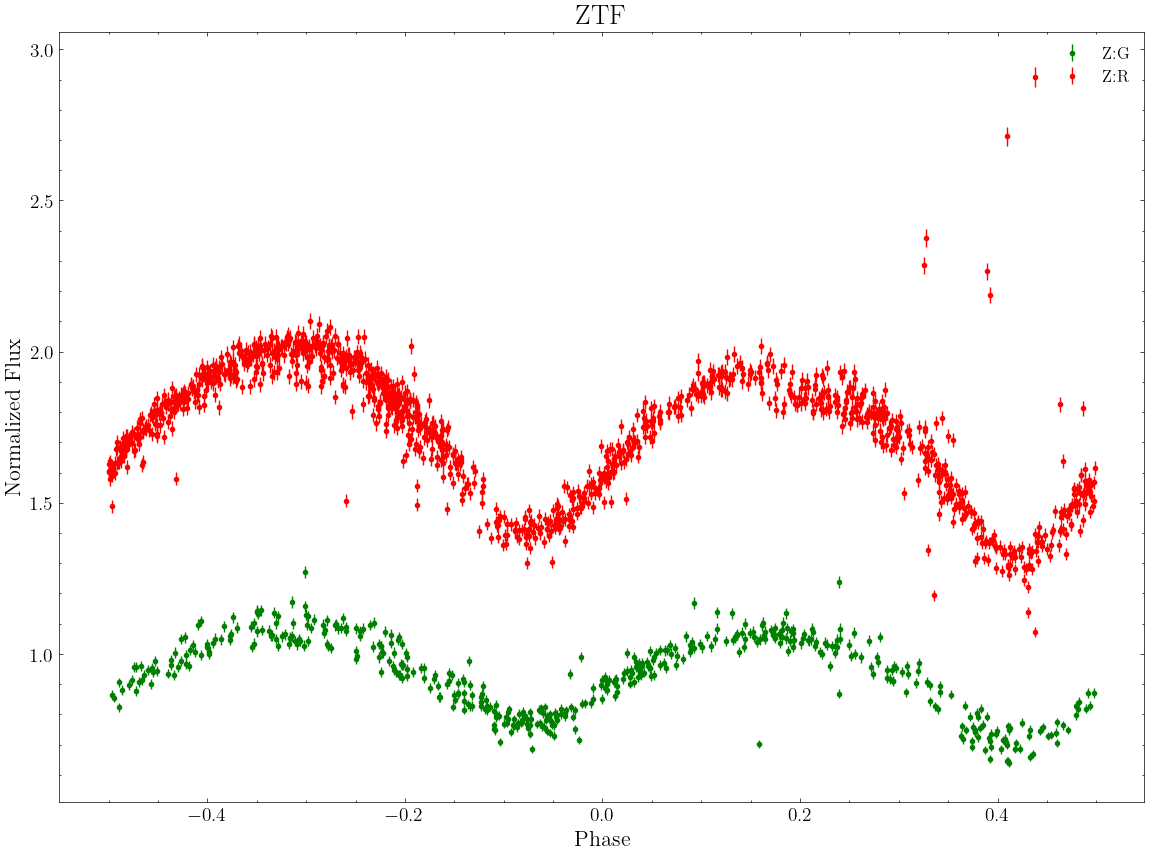
\includegraphics[scale=0.4]{Metodologia/Secciones/NormalizacionFlujos/Figures/ZTF Normalized Flux.png}
	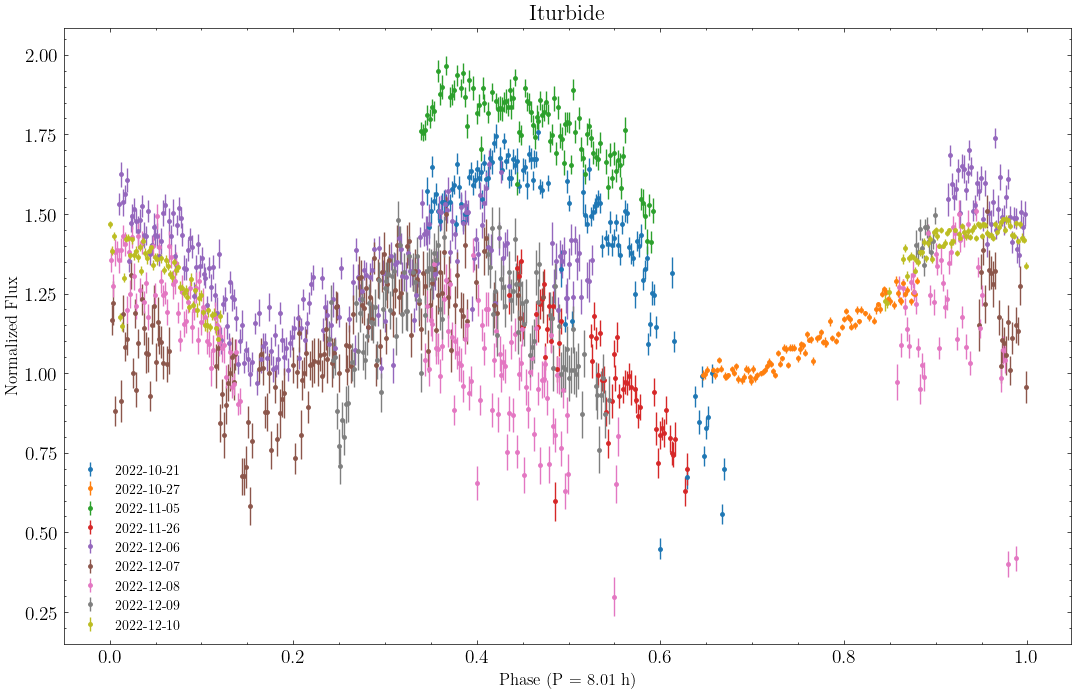
\includegraphics[scale=0.4]{Metodologia/Secciones/NormalizacionFlujos/Figures/Iturbide Normalized Flux.png}

	\caption{Flujo en fase de las curvas de luz obtenidas para \atoObjIdNoSpace.
	De estos dos conjuntos de datos solo ZTF contiene información del color del
	sistema, y por ende una cantidad medible del cual determinar la temperatura
	efectiva del sistema.}
	\label{figuraNormFlujosCurvas}
\end{figure}